\documentclass[12pt,oneside,a4paper]{article}
\usepackage{lastpage}
\usepackage{graphicx}
\usepackage{float}
\usepackage{fancyhdr}
\usepackage{xcolor}
\usepackage{color, colortbl}
\usepackage{colortbl}
\usepackage{xspace}
\usepackage{longtable}

% Colors Definition
\definecolor{link-blue}{RGB}{6,69,173}
\definecolor{dark-green}{RGB}{52,133,62}
\definecolor{light-green}{RGB}{93,186,105}
\definecolor{light-blue}{RGB}{127, 180, 240}
\definecolor{dark-blue}{RGB}{72, 120, 224}
\definecolor{heading-grey}{RGB}{181, 185, 189}
\definecolor{critical}{RGB}{173, 35, 10}
\definecolor{high}{RGB}{242, 93, 65}
\definecolor{medium}{RGB}{219, 173, 81}
\definecolor{low}{RGB}{235, 233, 113}
\definecolor{info}{RGB}{78, 142, 245}



\usepackage{hyperref}
\hypersetup{
    colorlinks = true,
    allcolors  = link-blue, 
}

% Variable Definition - Change Here
\newcommand{\companyName}{Company Name}
\newcommand{\companyNameShort}{CN}
\newcommand{\reportName}{Security Assessment Finding Report}
\newcommand{\pentester}{Sudneo Security}
\newcommand{\pentesterShort}{SSec}
\newcommand{\pentesterSite}{\url{https://coolbyte.eu}}


\pagestyle{fancy}
\fancyhf{}
\renewcommand{\footrulewidth}{0.3pt}
\rhead{\companyName}
\lhead{\reportName}
\rfoot{Page \thepage\ of \pageref*{LastPage}}
\cfoot{\companyName \\BUSINESS CONFIDENTIAL\\Copyright \copyright\xspace\textbf{\pentester}\ (\pentesterSite) }

\begin{document}
	\bgroup
	\begin{titlepage}
		\fancypagestyle{empty}{\fancyhf{}
		\renewcommand{\headrulewidth}{0pt}
		\fancyfoot[C]{\companyName\\BUSINESS CONFIDENTIAL\\Copyright \copyright\xspace\textbf{\pentester}\ (\pentesterSite)}}
		\begin{center}
			
\includegraphics[width=9cm]{images/logo.png}
			\linebreak\vspace{1cm}\linebreak
			{\huge\bfseries Company Name}\\
			% ----------------------------------------------------------------
			\vspace{1.0cm}
			{\Large\bfseries Security Assessment Finding Report}\\[5pt]
			% ----------------------------------------------------------------
			\vspace{2cm}
			{\Large \today}
		\end{center}
	\end{titlepage}
	\egroup
	\tableofcontents
	\newpage
	\section{Confidentiality Statement}
	This document is the exclusive property of \companyName\ (\companyNameShort) and \pentester\ (\pentesterShort). This document contains proprietary and confidential information. Duplication, redistribution, or use, in whole or in part, in any form, requires consent of both \companyNameShort\ and \pentesterShort.\\

	\noindent\pentesterShort\ may share this document with auditors under non-disclosure agreements to demonstrate penetration test requirement compliance.

	\section{Disclaimer}
	A penetration test is considered a snapshot in time.  The findings and recommendations reflect the information gathered during the assessment and not any changes or modifications made outside of that period.\\
	Time-limited engagements do not allow for a full evaluation of all security controls. \pentesterShort\ prioritized the assessment to identify the weakest security controls an attacker would exploit. \pentesterShort\  recommends conducting similar assessments on an annual basis by internal or third-party assessors to ensure the continued success of the controls.

	\section{Contact Information}
	\begin{table}[htpb]
	    \centering
	    \label{tab:contactInfo}
	    \begin{tabular}{|p{2cm}|p{2cm}|p{8.5cm}|}
		\hline
		\rowcolor{dark-blue}
		\textbf{Name} & \textbf{Title} & \textbf{Contact Information} \\ \hline
		\rowcolor{light-blue}
		\multicolumn{2}{|l|}{\companyName} & {} \\ \hline
		John Doe & CTO & Phone: 123456789\hfill\break Email: john@company.com \\ \hline 
		\rowcolor{light-blue}
		\multicolumn{3}{|l|}{\pentester} \\ \hline
		Sudneo & Pentester & Phone: 123456789\hfill\break Email: sudneo@sudneo.me \\ \hline
	    \end{tabular}
	\end{table}
	\pagebreak
	\section{Assessment Overview}
	From May 20th, 2019 to May 29th, 2019, \pentesterShort\ engaged \companyNameShort\ to evaluate the security posture of its infrastructure compared to current industry best practices that included an external penetration test.  All testing performed is based on the NIST SP 800-115 Technical Guide to Information Security Testing and Assessment, OWASP Testing Guide (v4), and customized testing frameworks. 
Phases of penetration testing activities include the following:
	\begin{itemize}
	\item Planning – Customer goals are gathered and rules of engagement obtained.
	\item  Discovery – Perform scanning and enumeration to identify potential vulnerabilities, weak areas, and exploits.
	\item Attack – Confirm potential vulnerabilities through exploitation and perform additional discovery upon new access.
	\item Reporting – Document all found vulnerabilities and exploits, failed attempts, and company strengths and weaknesses.
	\end{itemize}
	\begin{center}
	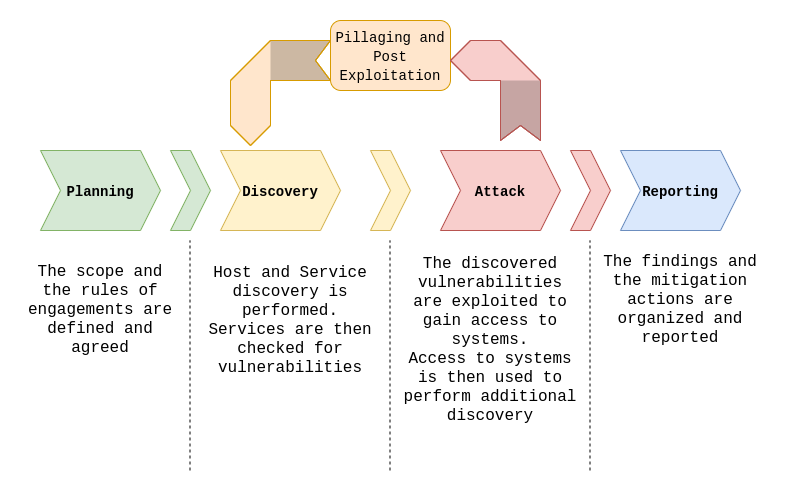
\includegraphics[width=\textwidth]{images/PentestCycle.png}
	\end{center}
	\pagebreak

	\section{Assessment Components}
	\label{sec:assessment_components}
	External Penetration Test

	An external penetration test emulates the role of an attacker attempting to gain access to an internal network without internal resources or inside knowledge.  A \pentesterShort engineer attempts to gather sensitive information through open-source intelligence (OSINT), including employee information, historical breached passwords, and more that can be leveraged against external systems to gain internal network access.  The engineer also performs scanning and enumeration to identify potential vulnerabilities in hopes of exploitation.	
	
	\section{Findings Severity Classification}
	\label{sec:findings_severity_classification}
    
	The following table defines levels of severity and corresponding CVSS score range that are used throughout the document to assess vulnerability and risk impact.
	
	\begin{table}[htpb]
	    \centering
	    \caption{Summary of the findings severity classification used.}
	    \label{tab:severityClassification}
	    \begin{tabular}{|p{2.5cm}|p{2.5cm}|p{9.5cm}|}
		\hline
		\multicolumn{1}{|>{\centering\arraybackslash}m{25mm}|}{\rowcolor{heading-grey}\textbf{Severity}}
    & \multicolumn{1}{>{\centering\arraybackslash}m{25mm}|}{\textbf{CVSS v3 Score Range}}
    & \multicolumn{1}{>{\centering\arraybackslash}m{95mm}|}{\textbf{Definition}}\\ \hline
		\cellcolor{critical}Critical & 9.0-10.0 & Exploitation is straightforward and usually results in system-level compromise.  It is advised to form a plan of action and patch immediately. \\ \hline
		\cellcolor{high}High & 7.0-8.9 & Exploitation is more difficult but could cause elevated privileges and potentially a loss of data or downtime.  It is advised to form a plan of action and patch as soon as possible. \\ \hline
		\cellcolor{medium}Moderate & 4.0-6.9 & Vulnerabilities exist but are not exploitable or require extra steps such as social engineering.  It is advised to form a plan of action and patch after high-priority issues have been resolved.  \\ \hline
		\cellcolor{low}Low & 0.1-3.9 & Vulnerabilities are non-exploitable but would reduce an organization’s attack surface.  It is advised to form a plan of action and patch during the next maintenance window.  \\ \hline
		\cellcolor{info}Informational & N/A & No vulnerability exists.  Additional information is provided regarding items noticed during testing, strong controls, and additional documentation.  \\ \hline
	    
	    \end{tabular}
	\end{table}
	\section{Scope}%
	\label{sec:scope}

	The overview of the scope of the engagement is described in Table \ref{tab:scopeEngagement}.

	Full details can be attached in Appendix.

	\begin{table}[htpb]
	    \centering
	    \caption{Scope of the engagement}
	    \label{tab:scopeEngagement}
	    \begin{tabular}{|p{5.5cm}|p{6.5cm}|}
	    \hline
	    \multicolumn{1}{|>{\centering\arraybackslash}m{55mm}|}{\rowcolor{heading-grey}\textbf{Assessment}} & \multicolumn{1}{>{\centering\arraybackslash}m{65mm}|}{\textbf{Details}} \\ \hline
	    External Penetration Test & 10.10.100.0/24 \hfill\break 10.100.10.0/24 \\ \hline
	    \end{tabular}
	\end{table}
	
	\subsection{Scope Exclusion}%
	\label{sub:scope_exclusion}
	
	Per client request, \pentesterShort\ did not perform any Denial of Service attacks during testing.

	\subsection{Client Allowances}%
	\label{sub:client_allowances}
	
	\comanyNameShort did not provide any allowances to assist the testing.
	\pagebreak
	
	\section{Executive Summary}%
	\label{sec:executive_summary}
	
	\pentesterShort\ evaluated \companyNameShort’s external security posture through an external network penetration test from May 20th, 2019 to May 29th, 2019.  By leveraging a series of attacks, \pentesterShort\ found critical level vulnerabilities that allowed full internal network access to the \companyNameShort\ headquarter office.  It is highly recommended that \companyNameShort\ address these vulnerabilities as soon as possible as the vulnerabilities are easily found through basic reconnaissance and exploitable without much effort.
	\subsection{Attack Summary}%
	\label{sub:attack_summary}
	

	The following table describes how \pentesterShort\ gained internal network access, step by step.

	\begin{table}[htpb]
	    \centering
	    \label{tab:attackSummary}
	    \begin{tabular}{|p{1cm}|p{5cm}|p{6cm}|}
		\hline
		\multicolumn{1}{|>{\centering\arraybackslash}m{10mm}|}{\rowcolor{heading-grey}\textbf{Step}}
    & \multicolumn{1}{>{\centering\arraybackslash}m{50mm}|}{\textbf{Action}}
    & \multicolumn{1}{>{\centering\arraybackslash}m{60mm}|}{\textbf{Recommendation}}\\ \hline
		1 & Perform port scan on \companyNameShort's infrastructure & Disable or protect ports which don't need to be public. \\ \hline
	    
	    \end{tabular}
	\end{table}

	\subsection{Security Strengths}%
	\label{sub:security_strengths}
	
	\paragraph{SIEM alerts of vulnerability scan}%
	\label{par:siem_alerts_of_vulnerability_scan}

	During the assessment, the \companyNameShort\ security team alerted \pentesterShort\ engineers of detected vulnerability scanning against their systems.  The team was successfully able to identify the \pentesterShort\  engineer’s attacker IP address within minutes of scanning and was capable of blacklisting \pentesterShort\ from further scanning actions.
	
	\subsection{Security Weaknesses}%
	\label{sub:security_weaknesses}
	
	\paragraph{Missing Password Policy}%
	\label{par:missing_password_policy}
	
	\pentesterShort\ successfully performed password attacks using lists of common passwords. Several systems of \companyNameShort\ were compromised using this method. Enabling a password policy that requires a minimum password complexity could protect the organization from similar attacks.

	\section{Vulnerabilities by Impact}%
	\label{sec:vulnerabilities_by_impact}
	
	Figure \ref{img:vulnerabilitiesbyimpact} illustrates the vulnerabilities found by impact.
	\begin{figure}[h]
	    \caption{Vulnerabilities by Impact}
	    \label{img:vulnerabilitiesbyimpact}
	    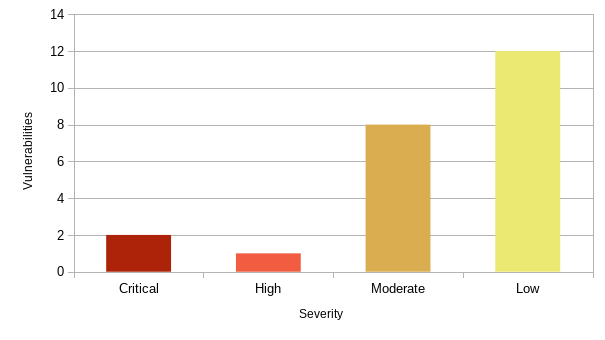
\includegraphics[width=\textwidth]{images/vulnsbyimpact.png} 
	\end{figure}


	\newpage
	\section{External Penetration Test Findings}%
	\label{sec:external_penetration_test_findings}
	
	\subsection{Insufficient Lockout Policy - Outlook Web App (Critical)}%
	\label{sub:insufficient_lockout_policy_outlook_web_app_critical_}
	
	\begin{table}[htpb]
	    \centering
	    \begin{tabular}{|p{3cm}|p{9cm}|}
		\hline
		\cellcolor{heading-grey}\textbf{Description:} & \companyNameShort\ allowed unlimited logon attempts against their Outlook Web App (OWA) services. This configuration allowed brute force and password guessing attacks in which \pentesterShort\ used to gain access to \companyNameShort\’s internal network. \\ \hline
		\cellcolor{heading-grey}\textbf{Impact:} & \cellcolor{critical}Critical \\ \hline
		\cellcolor{heading-grey} \textbf{System:} & 10.100.0.1 \\ \hline
	\cellcolor{heading-grey} \textbf{References:} & 
	\begin{itemize}
	    \item \href{https://nvd.nist.gov/800-53/Rev4/control/AC-17}{NIST SP800-53r4 AC-17} - Remote Access
	    \item \href{https://nvd.nist.gov/800-53/Rev4/control/AC-17}{NIST SP800-53r4 AC-7(1)} - Unsuccessful Logon Attempts; Automatic Account Lock
	\end{itemize} \\ \hline
	    \end{tabular}
	\end{table}

	\subsubsection{Exploitation Proof of Concept}%
	\label{ssub:exploitation_proof_of_concept}
	
	\pentesterShort\ gathered historical breached data found in credentials dumps.  The data amounted to 868 total account credentials (Note: A full list of compromised accounts can be found in “Demo Company-867-19 Full Findings.xslx”.).	

	\pentesterShort\ used the gathered credentials to perform a credential stuffing attack against the OWA login page.  Credential stuffing attacks take previously known credentials and attempt to use them on login forms to gain access to company resources.  \pentesterShort\ was unsuccessful in the attack but was able to gather additional sensitive information from the OWA server in the form of username enumeration.
	
	\subsubsection{Remediation}%
	\label{ssub:remediation}

	\begin{longtable}[htpb]{|p{2cm}|p{12cm}|}
	    \hline
	    \cellcolor{light-green}\textbf{Who:} & IT Team \\ \hline
	    \cellcolor{light-green}\textbf{Vector:} & Remote \\ \hline
	    \multicolumn{2}{|l|}{\cellcolor{light-green} \textbf{Actions:}} \\ \hline

	    1 & VPN and OWA login with valid credentials did not require Multi-Factor Authentication (MFA).  \pentesterShort\ recommends \companyNameShort\ implement and enforce MFA across all external-facing login services. \\ \hline 
	    2 & OWA permitted unlimited login attempts.  \pentesterShort\ recommends \companyNameShort\ restrict logon attempts against their service. \\ \hline
	    3 & \companyNameShort\ permitted a successful login via a password spraying attack, signifying a weak password policy.  \pentesterShort\ recommends the following password policy, per the Center for Internet Security (CIS):
		\begin{itemize}
		    \item 14 characters or longer
		    \item Use different passwords for each account accessed
		    \item Do not use words and proper names in passwords, regardless of language
		\end{itemize} \\ \hline
	    4 & OWA permitted user enumeration.\pentesterShort\ recommends \companyNameShort\ synchronize valid and invalid account messages. Additionally, \pentesterShort\ recommends that \companyNameShort\ :  
		\begin{itemize}
		    \item Train employees on how to create a proper password 
		    \item Check employee credentials against known breached passwords
		    \item Discourage employees from using work emails and usernames as login credentials to other services unless absolutely necessary
		\end{itemize} \\ \hline
	\end{longtable}

	\newpage
	\section{Additional Reports and Scans (Informational)}%
	\label{sec:additional_reports_and_scans_informational}
	
	\pentesterShort\ provides all clients with all report information gathered during testing.  This includes vulnerability scans and a detailed findings spreadsheet.  For more information, please see the following documents:
	\begin{itemize}
	    \item Demo Company-867-19 Full Findings.xslx
	    \item Demo Company-867-19 Vulnerability Scan Summary.xslx
	    \item Demo Company-867-19 Vulnerability Scan by Host.pdf
	\end{itemize}	
\end{document}
